% Abstract WAIMLAp 2026 — DINOv2 + LoRA on EuroSAT
% Compile with: pdflatex Abstract_DINOv2_EuroSAT_LoRA.tex (twice)
\documentclass[10pt,a4paper]{article}
\usepackage[utf8]{inputenc}
\usepackage[T1]{fontenc}
\usepackage{mathptmx}
\usepackage[scaled=0.92]{helvet}
\usepackage{courier}
\usepackage{amssymb}
\usepackage[a4paper,top=2.3cm,bottom=2.2cm,left=1.9cm,right=1.9cm,headsep=0.6cm,footskip=0.9cm]{geometry}
\usepackage{microtype}
\usepackage{booktabs}
\usepackage{tabularx}
\usepackage{caption}
\usepackage{graphicx}
\usepackage{fancyhdr}
\usepackage{xcolor}
\usepackage[hidelinks]{hyperref}
\usepackage{titlesec}

\definecolor{waimlap}{HTML}{4B2A82}

% ---- encabezado y pie del evento
\pagestyle{fancy}
\fancyhf{}
\renewcommand{\headrulewidth}{0pt}
\fancyhead[C]{\sffamily\small\color{waimlap}\textbf{Workshop on Artificial Intelligence and Machine Learning Applications}}
\fancyfoot[C]{\sffamily\footnotesize\color{waimlap}WAIMLAp 2026 \quad|\quad November 18--20, 2026 \quad|\quad Lima, Peru \quad|\quad waimlap.org}

% ---- secciones compactas
\titleformat{\section}{\normalfont\bfseries\small\uppercase}{\thesection.}{0.5em}{}
\titlespacing*{\section}{0pt}{0.9ex}{0.4ex}
\newcommand{\para}[1]{\textbf{#1}\enspace}
\setlength{\parindent}{0pt}
\setlength{\parskip}{0.45ex}
\captionsetup{font=small,labelfont=bf,skip=3pt}

\begin{document}

\begin{center}
{\large\bfseries Dissecting and Adapting DINOv2 for Land Cover Classification:\\[1pt]
An Architectural Teardown and Parameter-Efficient Study on Sentinel-2 Imagery\par}
\vspace{0.6em}
{\normalsize Alfredo Jiménez, Jhonatan Davila, Italo Ramos\par}
\vspace{0.2em}
{\small Departamento de Ingeniería, Pontificia Universidad Católica del Perú (PUCP), Lima, Peru\\
Grupo de Investigación en Inteligencia Artificial (IA-PUCP)\\
\texttt{alfredo.jf.2004@gmail.com}, \texttt{jcdavilam@pucp.edu.pe}, \texttt{italom.ramosd@pucp.edu.pe}\par}
\end{center}
\vspace{-0.4em}

\section{Introduction}
Self-supervised vision foundation models such as DINOv2~[1], a Vision Transformer (ViT)~[2] pre-trained on 142 million curated natural images, produce general-purpose features that transfer well with a frozen backbone. Satellite imagery, however, is a different domain: Sentinel-2 tiles~[3] are seen from above at about 10\,m per pixel, are dominated by repetitive textures, contain no central foreground object, and separate several classes only by subtle spectral differences. Linear probing (training a linear classifier on frozen features) is cheap and preserves the pre-trained representation, but cannot adapt it to remote-sensing textures; full fine-tuning updates all 22\,M parameters, is computationally costly and risks overfitting. We present an architectural teardown of DINOv2 ViT-S/14 and a controlled intervention with Low-Rank Adaptation (LoRA)~[4] restricted to the two deepest self-attention blocks. On the complete EuroSAT benchmark~[5] (27,000 images), evaluated on an NVIDIA Tesla T4 GPU, the intervention yields a statistically significant gain with a minimal parameter footprint and no measurable inference overhead.

\section{Methodology}
\para{Dataset and protocol.} We use EuroSAT RGB~[5] (Sentinel-2, 10 land-use and land-cover classes, 27,000 tiles of $64\times64$ px). Tiles are resized to $224\times224$ px with bicubic interpolation, which yields $16\times16$ patches of 14\,px; no center crop is applied, since it would remove 23\,\% of the scene. Images are normalized with ImageNet statistics, as in DINOv2 pre-training. A stratified 70/15/15 split with a fixed seed (42) gives 18,900 training, 4,050 validation and 4,050 test images. Following the DINOv2 linear evaluation protocol~[1], the classifier receives the concatenation of the [CLS] token and the mean of the patch tokens after the final LayerNorm (768 dimensions), giving a linear head of 7,690 parameters.

\para{Phase A: architectural teardown.} DINOv2 ViT-S/14 without registers~[6] has 22,056,576 parameters (88.2\,MB in fp32) in 12 identical Transformer blocks ($d=384$, 6 heads, MLP of 1,536 units). Each block holds 1.78\,M parameters (MLP 67\,\%, attention 33\,\%). The measured cost, which matches the analytical count, is 12.25\,GFLOPs per $224$\,px image (1.011\,GFLOPs per block, of which quadratic attention accounts for 9.9\,\%); at 448\,px it grows to 63.4\,GFLOPs (30.6\,\% attention). On the T4, latency is 8.89\,ms at batch 1 in fp32 (112.5\,img/s) and 1.17\,ms/img at batch 128 in fp16 (853.7\,img/s). The effective receptive field~[7] is global from block 1: the radius containing 50\,\% of the input gradient is 69.4\,px in block 1 and 85.0\,px in block 12 (90\,\%: 117.2\,px and 127.1\,px). A PCA of the patch tokens shows that block 4 mainly encodes patch position, whereas block 12 tokens group by semantic class.

\para{Phase B: LoRA intervention.} Since the semantic information concentrates in the last blocks, we keep blocks 1--10 frozen and add LoRA only to the query (Q) and value (V) projections of blocks 11 and 12. Each adapted weight becomes $W' = W + \frac{\alpha}{r} BA$, with $W$ frozen, $A \in \mathbb{R}^{8\times384}$ (Kaiming-uniform) and $B \in \mathbb{R}^{384\times8}$ initialized to zero ($r=\alpha=8$), so training starts exactly from the frozen model. This adds 24,576 trainable weights (0.11\,\% of the backbone; 32,266 or 0.146\,\% including the head). After training, $BA$ is merged into $W$. Both conditions use the same budget: AdamW~[8] (learning rate $10^{-3}$, weight decay $10^{-4}$), batch 64, 8 epochs, and model selection by validation macro-F1. The baseline trains on cached frozen embeddings (64\,s in total, including a single 61\,s extraction), while LoRA must back-propagate through blocks 11--12 (454\,s).

\section{Results and Discussion}
\para{Quantitative results.} On the 4,050 held-out test images (Table~1), LoRA raises macro-F1 from 95.80\,\% to 97.14\,\% (+1.34 percentage points) and accuracy from 96.00\,\% to 97.28\,\% (+1.28\,pp), reducing errors from 162 to 110 ($-32$\,\%). A McNemar test~[9] computed for the worst-case overlap of errors, a conservative bound, gives $\chi^2 = 9.56$, $p \approx 0.002$. After merging, inference cost is unchanged (4.43 vs.\ 4.41\,ms/img at batch 32).

\begin{table}[h]
\centering\small
\begin{tabularx}{\linewidth}{@{}Xrrrrr@{}}
\toprule
Method & Trainable params & \% of backbone & Test accuracy & Test macro-F1 & Test errors \\
\midrule
Linear probing (frozen DINOv2) & 7,690 & 0.035\,\% & 96.00\,\% & 95.80\,\% & 162 / 4,050 \\
LoRA (blocks 11--12, Q and V, $r=\alpha=8$) & 32,266 & 0.146\,\% & \textbf{97.28\,\%} & \textbf{97.14\,\%} & \textbf{110 / 4,050} \\
\bottomrule
\end{tabularx}
\caption{Performance on the EuroSAT test split (4,050 images, seed 42). Trainable parameters include the linear head.}
\end{table}
\vspace{-0.8em}

\para{Class-level analysis.} Every class improves its F1, and the largest gains occur on thin linear structures: Highway rises by 5.85\,pp (91.87\,\% to 97.72\,\%) and River by 3.71\,pp (93.80\,\% to 97.51\,\%); River tiles predicted as Highway drop from 21 to 2. Residential (+0.88\,pp) and Industrial (+0.57\,pp) also improve, while Forest and SeaLake stay above 98.8\,\%. The improvement is not uniform: new confusions appear among vegetation classes (PermanentCrop $\rightarrow$ HerbaceousVegetation, 1 to 13; Pasture $\rightarrow$ AnnualCrop, 2 to 10), so their recall decreases slightly while precision increases. These classes look alike at 64\,px in RGB, and the absence of near- and short-wave infrared bands likely contributes to this ambiguity. Figure~1 shows individual test predictions of both models.

\begin{figure}[h]
\centering
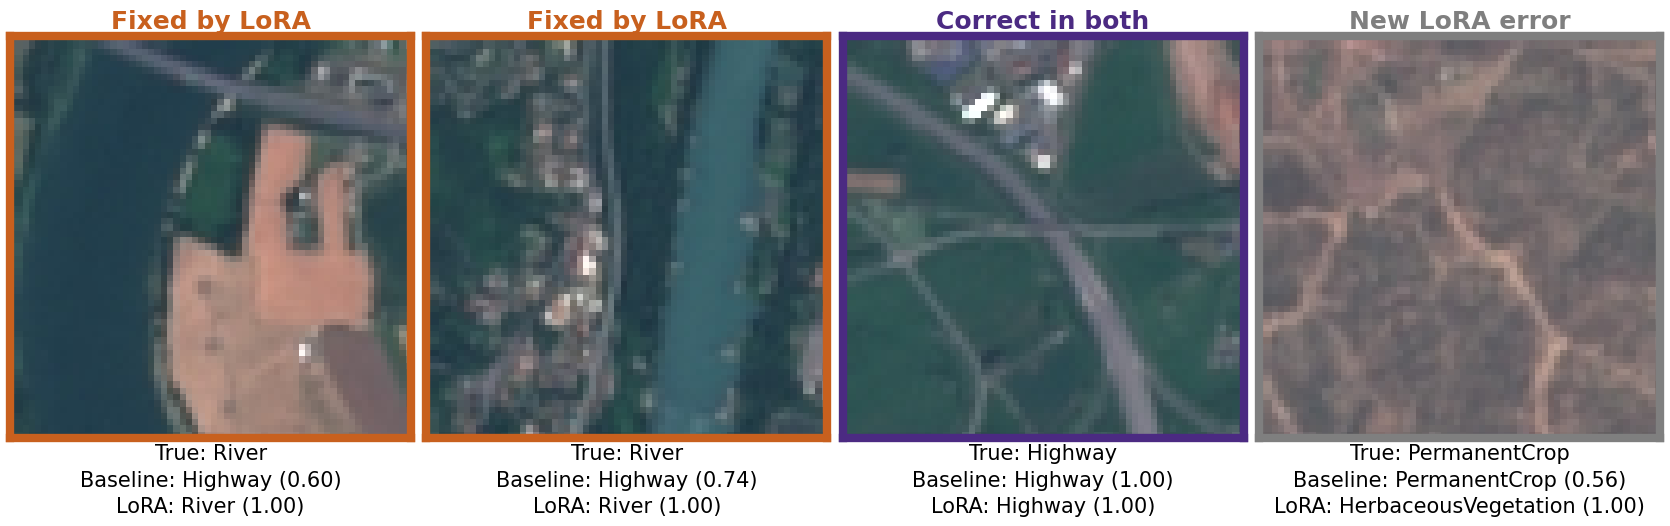
\includegraphics[width=0.92\linewidth]{fig_predicciones.png}
\caption{Individual test predictions with softmax probability. Two River tiles misclassified as Highway by linear probing are corrected by LoRA; a Highway tile is correct for both; a PermanentCrop tile becomes a new, confident LoRA error.}
\end{figure}
\vspace{-0.8em}

\section{Conclusions}
Adapting only the Q and V projections of the last two blocks of DINOv2 with LoRA (0.11\,\% of the backbone weights) narrows the gap between natural and satellite imagery, improving macro-F1 by 1.34\,pp ($p \approx 0.002$) with no extra inference cost after merging. Caching frozen embeddings makes the baseline inexpensive (one 61\,s extraction instead of re-encoding images every epoch), whereas LoRA training is about seven times slower.

\para{Limitations and Phase C.} The random stratified split measures in-distribution generalization only; neighboring tiles are spatially autocorrelated, which can inflate scores~[10]. Results come from a single seed. Phase C will evaluate both models on geographically disjoint regions built from the georeferenced EuroSAT multispectral GeoTIFFs, repeat the comparison with three seeds, and ablate the LoRA rank.

\section*{References}
\vspace{-0.3em}
{\footnotesize
\begin{enumerate}\setlength{\itemsep}{0pt}\setlength{\parskip}{0pt}\setlength{\leftskip}{-0.6em}
\renewcommand{\labelenumi}{[\arabic{enumi}]}
\item M. Oquab, T. Darcet, T. Moutakanni \emph{et al.}, ``DINOv2: Learning robust visual features without supervision,'' \emph{Transactions on Machine Learning Research (TMLR)}, 2024.
\item A. Dosovitskiy \emph{et al.}, ``An image is worth 16x16 words: Transformers for image recognition at scale,'' in \emph{Proc. ICLR}, 2021.
\item M. Drusch \emph{et al.}, ``Sentinel-2: ESA's optical high-resolution mission for GMES operational services,'' \emph{Remote Sensing of Environment}, vol.~120, pp.~25--36, 2012.
\item E. J. Hu \emph{et al.}, ``LoRA: Low-rank adaptation of large language models,'' in \emph{Proc. ICLR}, 2022.
\item P. Helber, B. Bischke, A. Dengel, and D. Borth, ``EuroSAT: A novel dataset and deep learning benchmark for land use and land cover classification,'' \emph{IEEE J. Sel. Topics Appl. Earth Observ. Remote Sens.}, vol.~12, no.~7, pp.~2217--2226, 2019.
\item T. Darcet, M. Oquab, J. Mairal, and P. Bojanowski, ``Vision transformers need registers,'' in \emph{Proc. ICLR}, 2024.
\item W. Luo, Y. Li, R. Urtasun, and R. Zemel, ``Understanding the effective receptive field in deep convolutional neural networks,'' in \emph{Proc. NeurIPS}, 2016.
\item I. Loshchilov and F. Hutter, ``Decoupled weight decay regularization,'' in \emph{Proc. ICLR}, 2019.
\item Q. McNemar, ``Note on the sampling error of the difference between correlated proportions or percentages,'' \emph{Psychometrika}, vol.~12, no.~2, pp.~153--157, 1947.
\item D. R. Roberts \emph{et al.}, ``Cross-validation strategies for data with temporal, spatial, hierarchical, or phylogenetic structure,'' \emph{Ecography}, vol.~40, no.~8, pp.~913--929, 2017.
\end{enumerate}}

\end{document}
